\documentclass[landscape]{article}
\usepackage{multicol}
\usepackage{calc}
\usepackage{ifthen}
\usepackage[landscape]{geometry}
\usepackage{amsmath,amsthm,amsfonts,amssymb}
\usepackage{color,graphicx,overpic}
\usepackage[bookmarks=false]{hyperref}
\usepackage{wrapfig}
\usepackage{eso-pic}
\usepackage[defaultfam,tabular,lining]{montserrat} 
\usepackage{float}
\usepackage{tabularx}
%\usepackage[dvipsnames, table]{xcolor}
\usepackage{blindtext}
\usepackage{multirow}
\usepackage{listings}
\usepackage[x11names]{xcolor}
%\usepackage[dvipsnames]{xcolor}
\usepackage{pythonhighlight}
\usepackage{ragged2e}
%\geometry{legalpaper, landscape, margin=0.5in}
\pdfinfo{
  /Title (PyAnsys Cheat sheet)
  /Creator (TeX)
  /Producer (pdfTeX 0.XX.1)
  /Author (Ansys Inc.,)
  /Subject (PyAEDT)
  /Keywords (PyAEDT,AEDT,ANSYS)}

% This sets page margins to .5 inch if using letter paper, and to 1cm
% if using A4 paper. (This probably isn't strictly necessary.)
% If using another size paper, use default 1cm margins.
\ifthenelse{\lengthtest { \paperwidth = 11in}}
    { \geometry{top=.15in,left=.25in,right=.25in,bottom=.1in} }
    {\ifthenelse{ \lengthtest{ \paperwidth = 297mm}}
        {\geometry{top=1cm,left=1cm,right=1cm,bottom=1cm} }
        {\geometry{top=1cm,left=1cm,right=1cm,bottom=1cm} }
    }

% Turn off header and footer
\pagestyle{empty}

% Redefine section commands to use less space
\makeatletter
\renewcommand{\section}{\@startsection{section}{1}{0mm}%
                                {-1ex plus -.5ex minus -.2ex}%
                                {0.5ex plus .2ex}%x
                                {\normalfont\large\bfseries}}
\renewcommand{\subsection}{\@startsection{subsection}{2}{0mm}%
                                {-1explus -.5ex minus -.2ex}%
                                {0.5ex plus .2ex}%
                                {\normalfont\normalsize\bfseries}}
\renewcommand{\subsubsection}{\@startsection{subsubsection}{3}{0mm}%
                                {-1ex plus -.5ex minus -.2ex}%
                                {1ex plus .2ex}%
                                {\normalfont\small\bfseries}}
\makeatother

\definecolor{silver}{RGB}{217,216,214}
\definecolor{gold}{RGB}{255,183,27}
\definecolor{steel}{RGB}{137,138,141}
\definecolor{lead}{RGB}{55,58,54}
\definecolor{bronze}{RGB}{200,146,17}
\definecolor{cblack}{RGB}{0,0,0}
\definecolor{codegreen}{rgb}{0,0.6,0}
\definecolor{codegray}{rgb}{0.5,0.5,0.5}
\definecolor{codepurple}{rgb}{0.58,0,0.82}

\lstdefinestyle{python_style}{
	backgroundcolor=\color{white},
	%commentstyle=\color{white},
	%keywordstyle=\color{gold},
	%stringstyle=\color{cblack}
	%backgroundcolor=\color{backcolour},   
	commentstyle=\color{codegreen},
	keywordstyle=\color{magenta},
	numberstyle=\tiny\color{codegray},
	stringstyle=\color{codepurple},
	frame=single,
	breaklines,
	%basicstyle=\sffamily\footnotesize,
	basicstyle=\ttfamily,
	showspaces=false,
	showstringspaces=false,
    	showtabs=false,
	%tabsize=2
}

\lstset{style=python_style}

\def\code#1{\texttt{#1}}

% Define BibTeX command
\def\BibTeX{{\rm B\kern-.05em{\sc i\kern-.025em b}\kern-.08em
    T\kern-.1667em\lower.7ex\hbox{E}\kern-.125emX}}

% Don't print section numbers
\setcounter{secnumdepth}{0}


\setlength{\parindent}{0pt}
\setlength{\parskip}{0pt plus 0.5ex}

%My Environments
\newtheorem{example}[section]{Example}
% -----------------------------------------------------------------------

\begin{document}
%\raggedright
\footnotesize
\justifying
\begin{center}
     \Huge{\textbf{PyAEDT-API Cheat sheet}} \\
\end{center}
\AddToShipoutPicture*
{\put(670,577.5){
\includegraphics[height = 1.2cm]{ansys.png}}}
\AddToShipoutPictureBG*{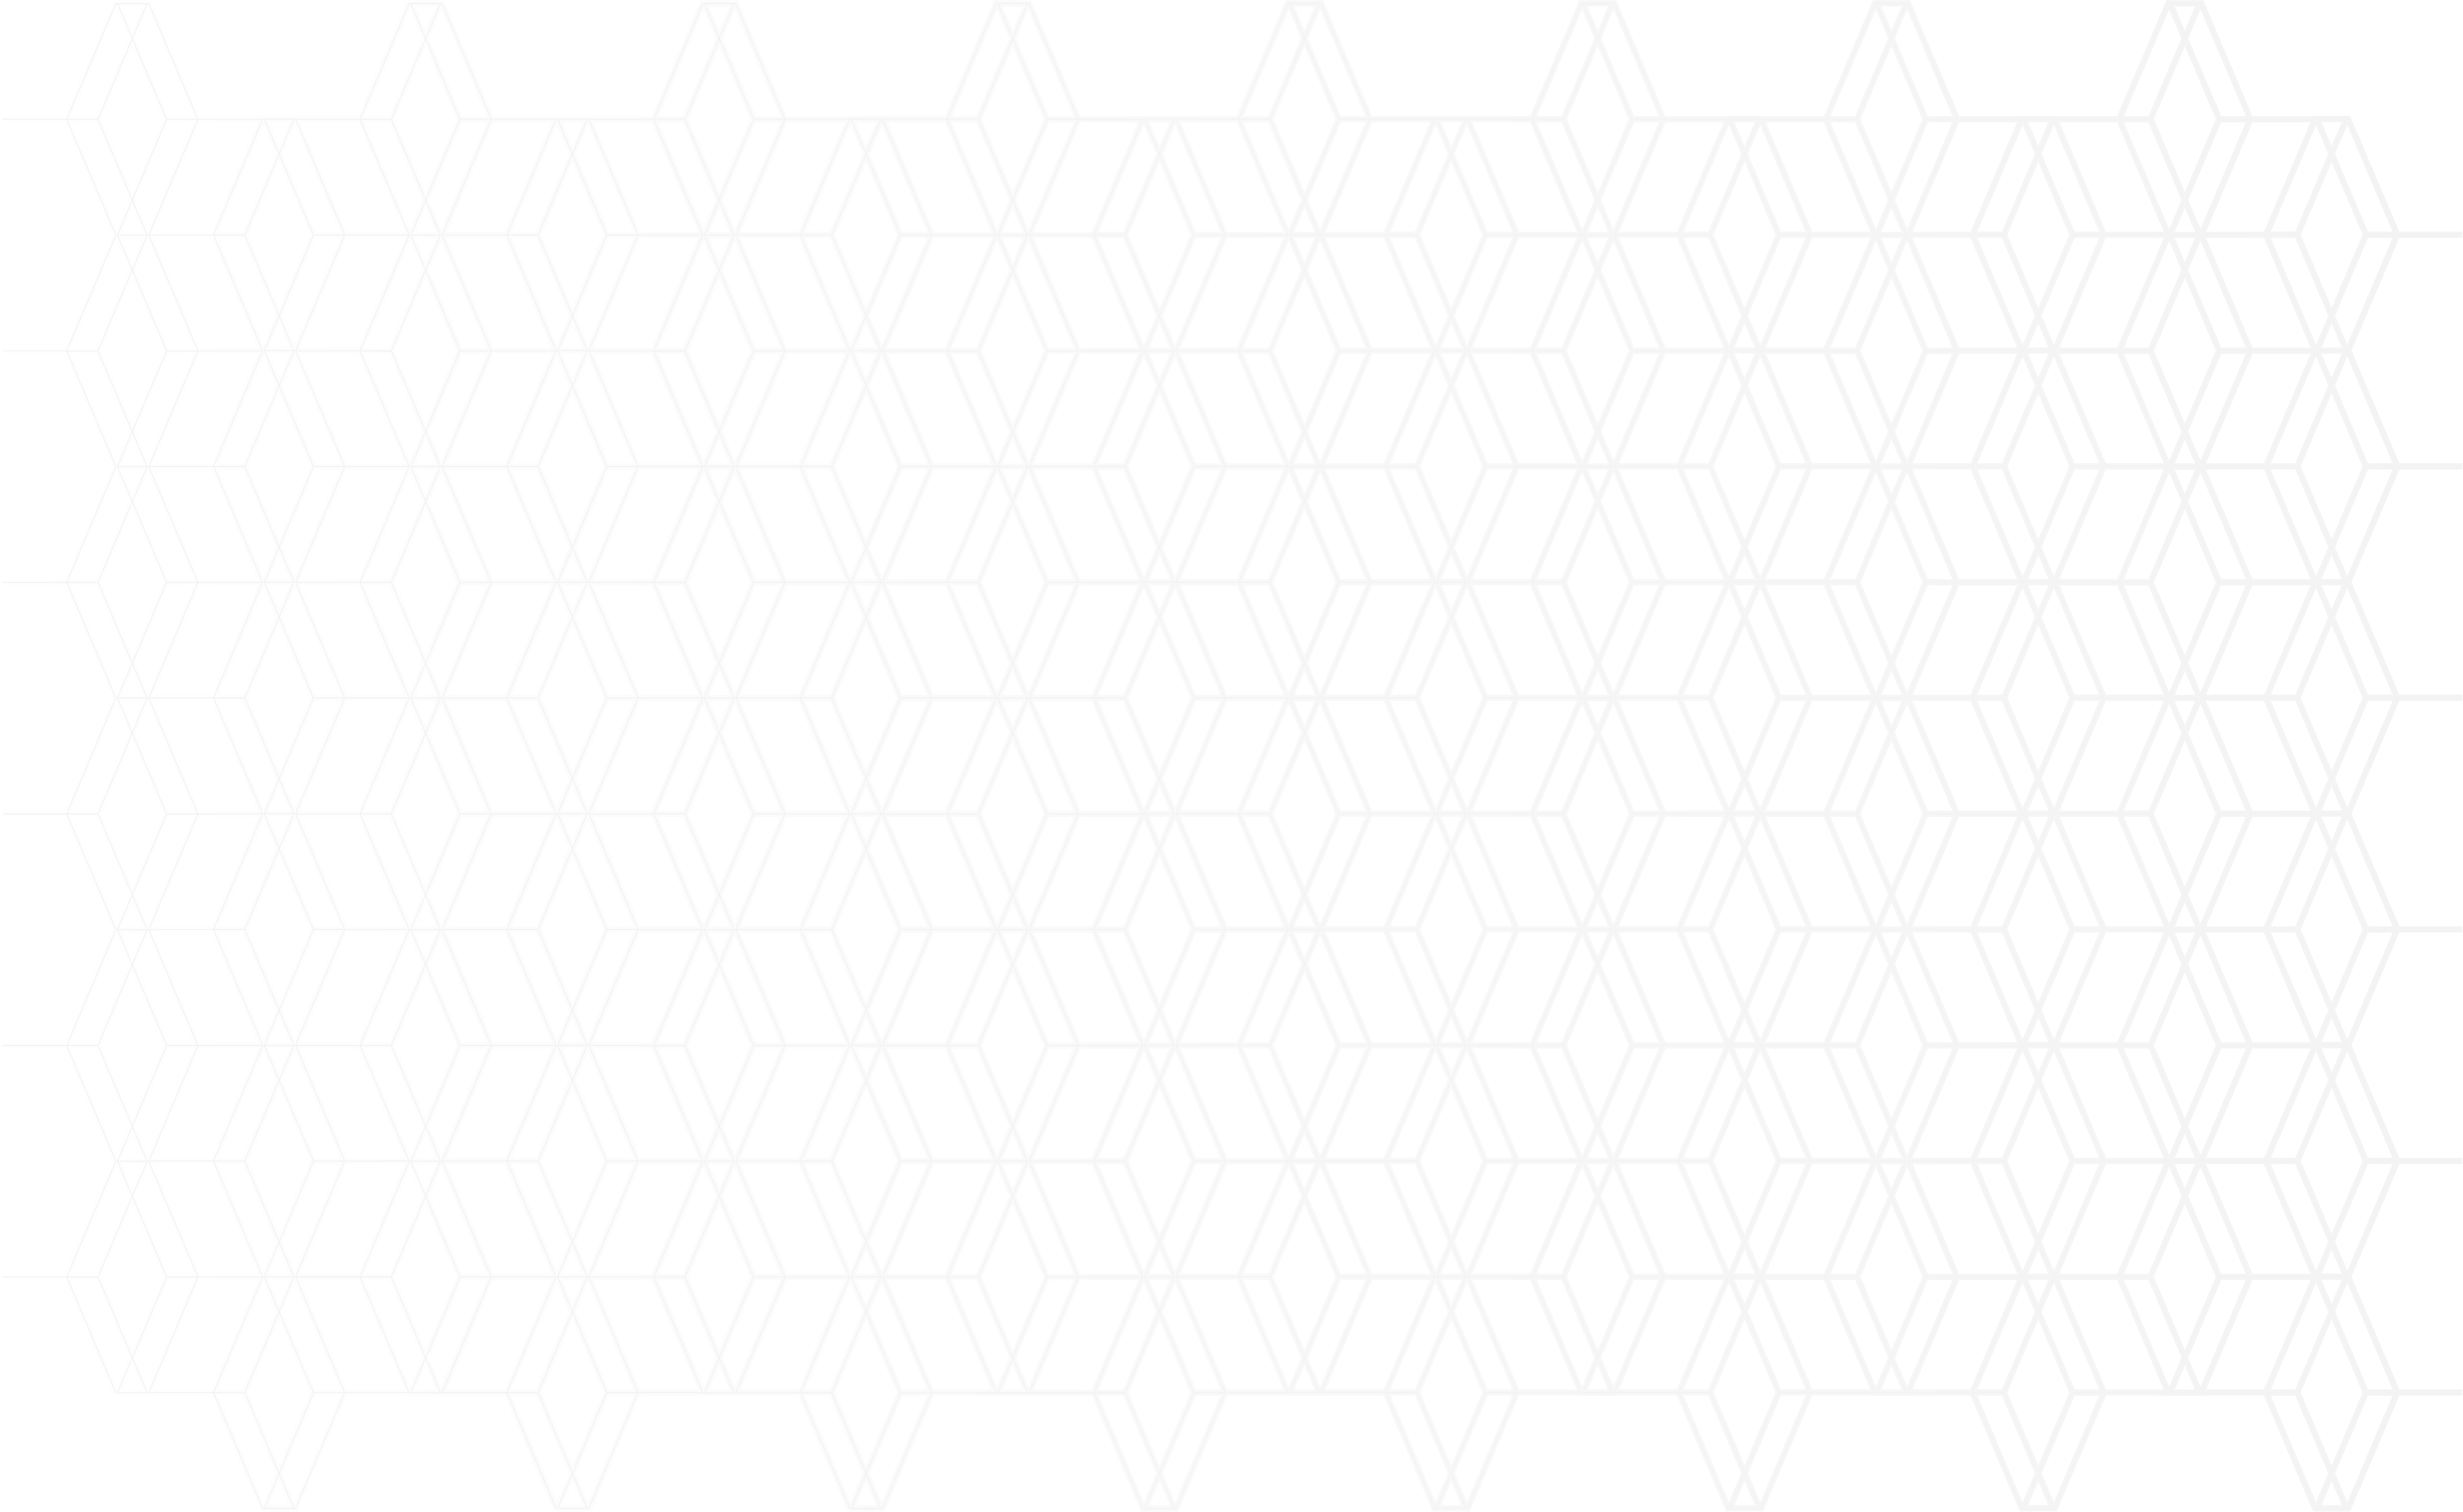
\includegraphics[width=\paperwidth]{bground_2.png}}
\vspace{-0.15cm}
\noindent\makebox[\linewidth]{\rule{\paperwidth}{2pt}}

\begin{multicols}{3}
% multicol parameters
% These lengths are set only within the two main columns
%\setlength{\columnseprule}{0.25pt}
\setlength{\premulticols}{1pt}
\setlength{\postmulticols}{1pt}
\setlength{\multicolsep}{1pt}
\setlength{\columnsep}{2pt}

\section{
\includegraphics[height=\fontcharht\font`\S]{slash.png} Launching PyAEDT}
To launch HFSS instance locally and exit it
\begin{lstlisting}[language=Python]
# To launch an instance
import pyaedt
hfss = pyaedt.Hfss(specified_version="2023.1",
	non_graphical=False,
	new_desktop_session=True, 
	projectname="Project_name",
	designname="Design_name")
# To exit the instance
hfss.release_desktop()
\end{lstlisting}

%Optionally, AEDT can be launched at the client server. To connect an existing instance of AEDT at  \textbf{"server\_name"} and port \textbf{"50001"}
%\begin{lstlisting}[language=Python]
%	cl1 = create_session("server_name", launch_aedt_on_server=True, 
%	aedt_port=50001, non_graphical=True)
%\end{lstlisting}


\section{
\includegraphics[height=\fontcharht\font`\S]{slash.png} Variable Class}
Creating a local and global variable in HFSS
\begin{lstlisting}[language=Python]
hfss["dim"] = "1mm"   # design variable
hfss["$dim"] = "1mm"  # project variable
\end{lstlisting}
\texttt{hfss.variable$\_$manager} is the class handles all the variables. It contains a lot of properties and methods useful for variable handling.
\section{
\includegraphics[height=\fontcharht\font`\S]{slash.png} Material Class}
\texttt{hfss.materials} class is used to access the material library. A new material is added in HFSS as
\begin{lstlisting}[language=Python]
my_mat = hfss.materials.add_material("myMat")
my_mat.permittivity = 3.5
my_mat.conductivity = 450000
my_mat.permeability = 1.5
\end{lstlisting}
%A python dictionary of material properties can be added while adding the material itself.
%\begin{lstlisting}[language=Python]
%dic = {"permittivity":4.5, "permeability":1.5,  "conductivity":45000}
%my_mat = hfss.materials.add_material("myMat2", props = dic)
%\end{lstlisting}  

\section{
\includegraphics[height=\fontcharht\font`\S]{slash.png} Geometry Creation}
\texttt{hfss.modeler} contains all properties and methods needed to edit a modeler, including primitives methods and properties.
\newline
\\
A box is drawn at (x\_pos, y\_pos, z\_pos) position with (x\_dim, y\_dim, z\_dim) dimensions as
\begin{lstlisting}[language=Python]
box = hfss.modeler.create_box([x_pos,y_pos,z_pos], [x_dim,y_dim,z_dim],name="airbox", matname="air")
\end{lstlisting}

A spiral geometry made of "copper" is created as follows

\begin{lstlisting}[language=Python]
ind = hfss.modeler.create_spiral(
	internal_radius=rin, width=width,
	spacing=spacing, turns=Nr,
	faces=Np, thickness=thickness,
	material="copper",name="Inductor1")
\end{lstlisting}
\texttt{box}, \texttt{ind} are the \texttt{Object3d objects}, containing a lot of properties and methods related to that object including faces, vertices, colors, and materials.
\columnbreak

\section{
\includegraphics[height=\fontcharht\font`\S]{slash.png} Creating boundaries}
In AEDT, open region is created as 
\begin{lstlisting}[language=Python]
hfss.create_open_region(Frequency="1GHz")
\end{lstlisting}
Assigning the radiation boundary to a box is as follows
\begin{lstlisting}[language=Python]
hfss.assign_radiation_boundary_to_objects("airbox") 
\end{lstlisting}

\section{
\includegraphics[height=\fontcharht\font`\S]{slash.png} Port definitions}
Common port types in HFSS are Lumped-port and Wave guide-port. Pythonic way of defining the lumped-port is
\begin{lstlisting}[language=Python]
box1 = hfss.modeler.create_box([0,0,50], [10,10,5], "Box1","copper")
box2 = hfss.modeler.create_box([0,0,60], [10,10,5], "Box2","copper")
port_L = hfss.lumped_port(signal="Box1", reference="Box2", integration_line=hfss.AxisDir.XNeg, impedance=50, name="LumpedPort", renormalize=True, deembed=False)
\end{lstlisting}

Pythonic way of defining Wave guide-port is 
\begin{lstlisting}[language=Python]
port_W = hfss.wave_port("Box1","Box2",name="WavePort",integration_line=1)
\end{lstlisting}



\section{
\includegraphics[height=\fontcharht\font`\S]{slash.png} Setup Class}
Setup class is used to define the solution setup in the PyAEDT

\begin{lstlisting}[language=Python]
setup = hfss.create_setup("MySetup")
setup.props["Frequency"] = "50MHz"
setup["MaximumPasses"] = 10
hfss.create_linear_count_sweep(setupname="any",unit="MHz",freqstart=0.1,freqstop=100,num_of_freq_points=100, sweepname="sweep1",sweep_type="Interpolating", save_fields=False)
\end{lstlisting}

Parametric sweep and optimizations are accessed using following classes

\begin{lstlisting}[language=Python]
# returns the ParametericsSetups Class
hfss.parametrics
# returns the OptimizationSetups Class
hfss.optimizations
\end{lstlisting}
\columnbreak
\section{
\includegraphics[height=\fontcharht\font`\S]{slash.png} Mesh Class}
Mesh module manages the mesh functions in PyAEDT
\begin{lstlisting}[language=Python]
hfss.mesh.assign_initial_mesh_from_slider(level=6) # setting the slider level to 6
# assign model resolutions
hfss.mesh.assign_model_resolution(names=[object1.name, object2.name], defeature_length=None)
# assigning the mesh length to the object1 faces
hfss.mesh.assign_length_mesh(names=object1.faces, isinside=False, maxlength=1, maxel=2000)
\end{lstlisting}

\section{
\includegraphics[height=\fontcharht\font`\S]{slash.png} Analysis Class}
The solution setup (\texttt{mysetup}) in HFSS design is analyzed by calling the following Python command 
\begin{lstlisting}[language=Python]
hfss.analyze_setup("mysetup")
\end{lstlisting}
%where, 'mysetup' is the solution setup
\section{
\includegraphics[height=\fontcharht\font`\S]{slash.png} Post-processing Class}
Post-processing class has modules for creating and editing plots in AEDT. They are accessible through the post library
\begin{lstlisting}[language=Python]
plotf = hfss.post.create_fieldplot_volume(object_list, quantityname, setup_name, intrinsic_dict) # This call return a FieldPlot object
my_data = hfss.post.get_solution_data(expression=trace_names) # This call return a SolutionData object
standard_report = hfss.post.report_by_category.standard("db(S(1,1))") # This call returns a new standard report object
standard_report.create() # This call reate a report
solution_data = standard_report.get_solution_data()
\end{lstlisting}

\section{
\includegraphics[height=\fontcharht\font`\S]{slash.png} Calling AEDT-API with PyAEDT}
Most of the critical functionalities are captured in PyAEDT. However, the missing features from AEDT-API method can be converted to PyAEDT method.
\newline
\\
Example: AEDT-API module (\texttt{Optimetrics}), is accessible in PyAEDT as
\begin{lstlisting}[language=Python]
omodule = hfss.odesign.GetModule("Optimetrics")
\end{lstlisting}

\subsection{References from PyAEDT Documentation}
\begin{itemize}
\item \href{https://aedt.docs.pyansys.com}{Getting Started}
%\item \href{https://aedt.docs.pyansys.com/release/0.6/User_guide/index.html}{User Guide}
%\item \href{https://aedt.docs.pyansys.com/release/0.6/API/index.html}{API Reference}
\end{itemize}
\end{multicols}
\vspace{-0.5cm}
\noindent\makebox[\linewidth]{\rule{\paperwidth}{4pt}}
\begin{center}
Getting Started With AEDT 
\includegraphics[height=\fontcharht\font`\S]{slash.png} Ansys Innovation Courses 
\includegraphics[height=\fontcharht\font`\S]{slash.png} %Visit \code{\href{https://courses.ansys.com/}{ansys.com/courses}}
\end{center}
\end{document}
